\documentclass[12pt]{article}

\usepackage{amsfonts, amsmath, amssymb, amstext, latexsym}
\usepackage{graphicx, epsfig}
\usepackage[latin1]{inputenc}
\usepackage[french]{babel}
\usepackage{exscale}
\usepackage{amsbsy}
\usepackage{amsopn}
\usepackage{fancyhdr}
\usepackage{float}
\newcommand{\noi}{\noindent}
\newcommand{\dsp}{\displaystyle}
\newcommand{\ind}{{{\large 1} \hspace*{-1.6mm} {\large 1}}}


\textheight 25cm
\textwidth 16cm
\oddsidemargin 0cm
\evensidemargin 0cm
\topmargin 0cm
\hoffset -0mm
\voffset -20mm


\pagestyle{plain}



% titre, auteur et date
\title{TP Principes et M\'{e}thodes Statistiques}
\author{Gabriel Sarrazin, Nejmeddine Douma, Simon Rabourg}
\date{Avril 2015}

% le debut du contenu
%===============
\begin{document}
%===============

% pour afficher titre, auteur et date
\maketitle

\section{Analyse des d\'{e}fauts de cuves}


\section{V\'{e}rifications exp\'{e}rimentales \`{a} base de simulations}


\begin{enumerate}
\item Il est possible de simuler n \'{e}chantillons de la loi Pa(a,b) car nous connaissons sa fonction de r\'{e}partiton. 
\\
$P_a(a,b)$ est une fonction continue, elle peut donc s'apparenter \`{a} une loi uniforme.  Dans un premier temps, simuler n \'{e}chantillons de cette loi va donc consister  \`{a} tirer, au hasard, n valeurs al\'{e}atoires sur l'intervalle [0,1]. Connaissant la fonction de r\'{e}partition de la loi  $P_a(a,b)$,nous allons ensuite calculer l'image inverse $ F^{-1}(Ui)$  pour obtenir un \'{e}chantillon de loi $P_a(a,b)$ et nous ferons cela pour les n valeurs obtenues sur [0,1].
\\
$$ U = 1 - b^a/ F^{-1}(U)^a$$
$$ \Longrightarrow -F^{-1}(U)^a = -b^a/ U-1$$
$$ \Longrightarrow F^{-1}(U)^a = b^a/ 1-U$$
$$  \Longrightarrow-F^{-1}(U) = b/ (1-U)^{(1/a)}$$
\\
Nous pouvons repr\'{e}senter cette m\'{e}thode sous forme d'un graphique : en mettant en ordonn\'{e}e les n valeurs de la loi Ui et en abscisse la projection pour chacune de ses valeurs de son image inverse ($F^{-1}(Ui)$ ).
\\

\item
 En suivant la m\'{e}thode d\'{e}crite pr\'{e}cedemment, nous  avons simuler m \'{e}chantillon de taille n avec diff\'{e}rentes valeurs pour m,n et a. 
\\
Nous avons ensuite, pour chaque \'{e}chantillon de taille n, calculer l'intervalle de confiance bilat\'{e}ral. Pour cela nous avons utiliser L'intervalle de confiance trouv\'{e} en premi\`{e}re partie qui s'utilise avec $Y=\ln {\dsp \frac{X}{2}}$.  A chaque fois que a est bien contenu dans cet intervalle, nous inc\'{e}mentons une variable compteur. La proportion Pr d'IC contenant a est donc $Pr = Compteur/m$.
\\

\begin{figure}[H]
\label{graph1}
\centering
\includegraphics[width=1.0\textwidth]{figures/Graph_P2Q2.pdf}
\caption{Graphe des proportions d'IC($\alpha$) contenant la valeur exacte de a pour diff\'{e}rentes valeurs de $\alpha$}
\end{figure}

Afin que cela soit plus repr\'{e}sentatif,nous avons trac\'{e} un graphique avec les diff\'{e}rentes proportions obtenues en fonction des $\alpha$. (Voir figure page \ref{graph1})
\\

Nous pouvons voir qu'il existe une lin\'{e}arit\'{e} entre la proportion et les $\alpha$. Plus on augmente le nombre d'\'{e}chantillon m et leur taille n et plus l'approximation est exacte. Ces points ont \'{e}t\'{e} obtenus pour les valeurs de $m = 100$, $n = 10, 30, 50, 100, 200, 500$, $a = 3, 5, 10, 20, 50$ et $\alpha = 0.01, 0.05, 0.10, 0.20 ..., 0.80, 0.90, 0.95, 0.99$.
\\
Quand on simule un grand nombre m d\'{e}chantillons de taille $n$ de la  loi $P_a(a,2)$ alors la proportion d'IC($\alpha$) contenant $a$ est aproximativement \'{e}gale \`{a}  $1 - \alpha$.
\\

\item

 Afin d'estimer le param\`{e}tre $a$, nous disposons de trois m\'{e}thodes : la m\'{e}thode des moments, la m\'{e}thode du maximum de vraisemblance qui nous m\`{e}nent au m\^{e}me r\'{e}sultat pour l'\'{e}stimation du param\`{e}tre $a$ et nous pouvons aussi d\'{e}terminer l'estimateur sans bais de variance minimale si celui-ci existe.
\\

\begin{figure}[H]
\centering
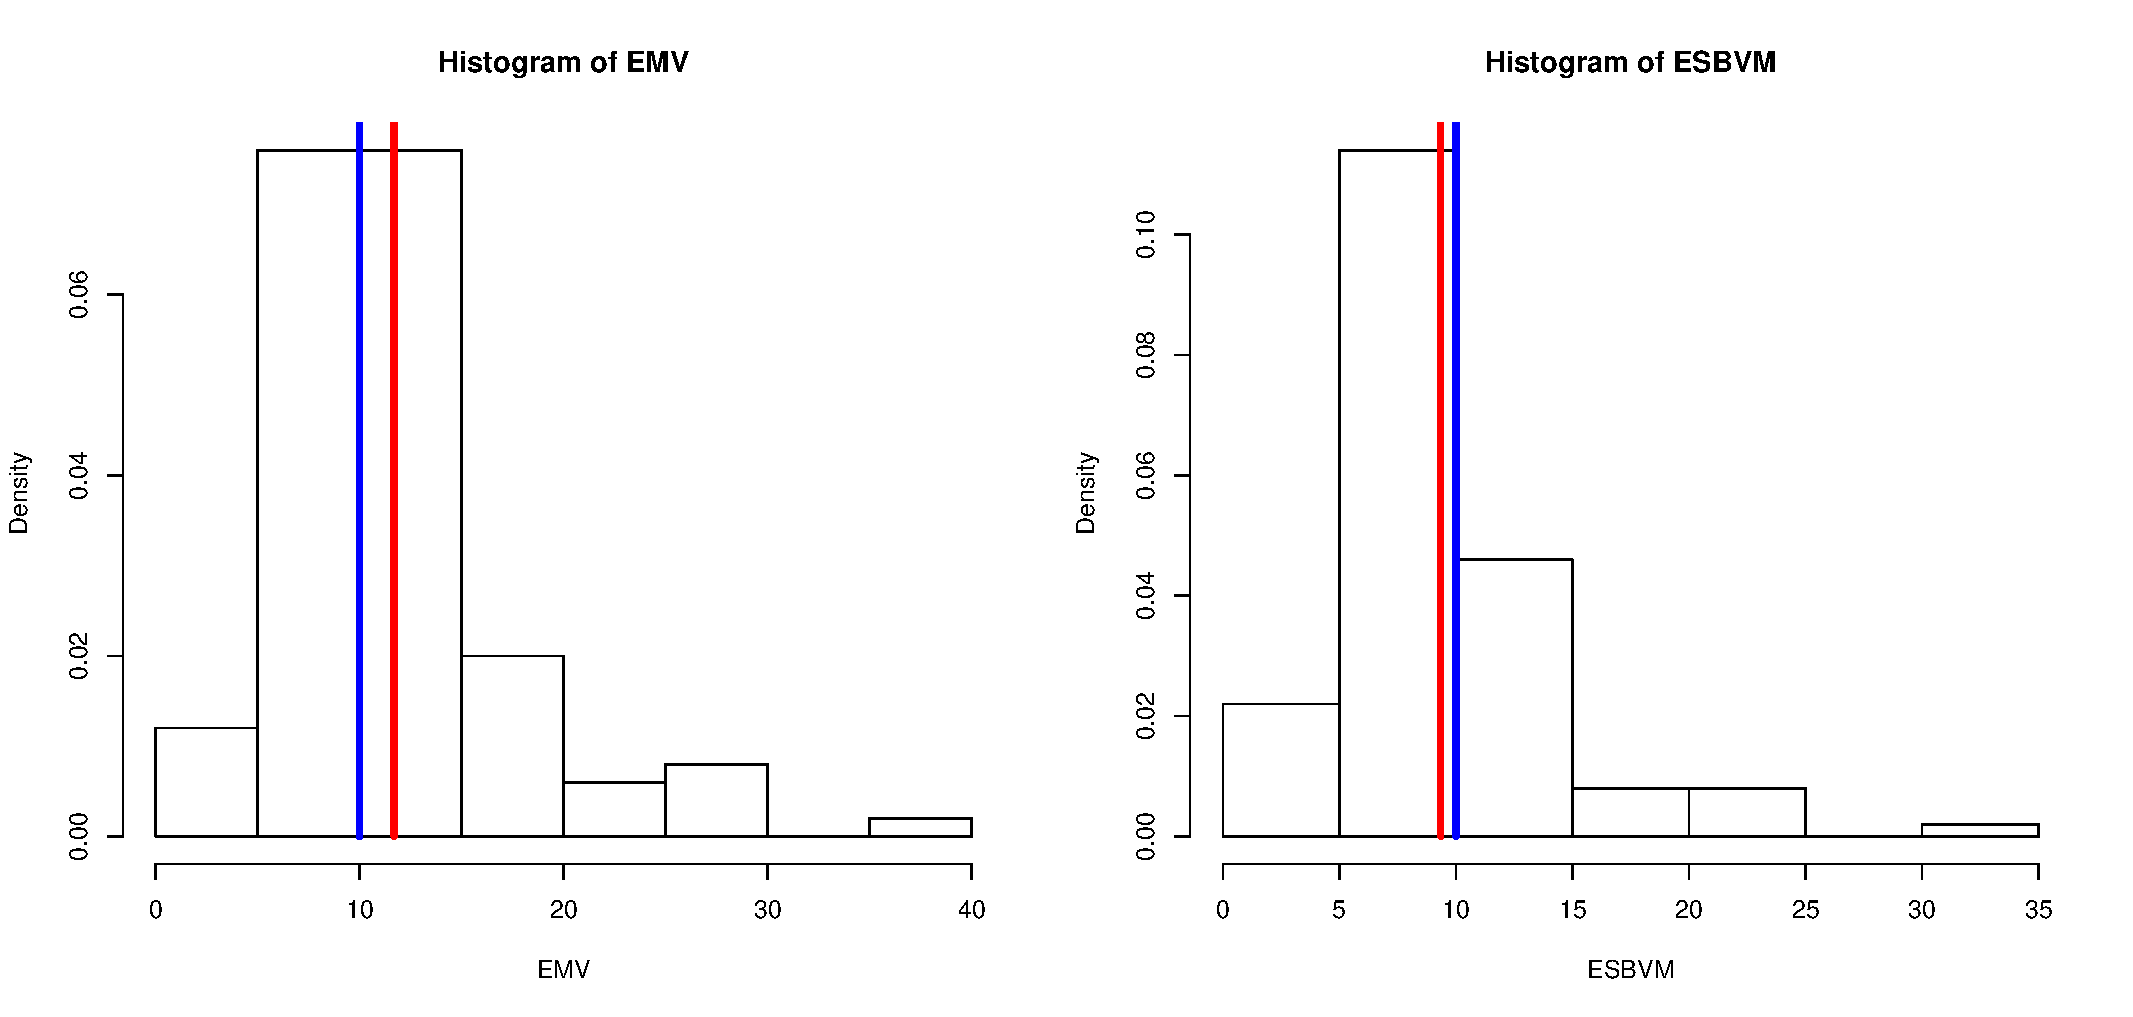
\includegraphics[width=1.0\textwidth]{figures/GraphP2Q31.pdf}
\caption{Histogramme des EMV et ESBVM pour $m=100, n=5, a=10$}
\label{graphe2}
\end{figure}

\begin{figure}[H]
\centering
\includegraphics[width=1.0\textwidth]{figures/GraphP2Q32.pdf}
\caption{Histogramme des EMV et ESBVM pour $m=100, n=20,   a=10$}
\label{graph3}
\end{figure}

\begin{figure}[H]
\centering
\includegraphics[width=1.0\textwidth]{figures/GraphP2Q33.pdf}
\caption{Histogramme des EMV et ESBVM pour $m=100, n=50, a=10$}
\label{graphe4}
\end{figure}

\begin{figure}[H]
\centering
\includegraphics[width=1.0\textwidth]{figures/GraphP2Q34.pdf}
\caption{Histogramme des EMV et ESBVM pour $m=100, n=100, a=10$}
\label{graphe5}
\end{figure}

\begin{figure}[H]
\centering
\includegraphics[width=1.0\textwidth]{figures/GraphP2Q35.pdf}
\caption{Histogramme des EMV et ESBVM pour $m=500, n=5, a=10$}
\label{graphe6}
\end{figure}

Pour chaque \'{e}chantillons (m en tout) nous avons mis au point sur R une fonction qui calcule les estimateurs propos\'{e}s , qui estime le biais et l'erreur quadratique de chaque estimateur, et qui fait une moyenne pour chacun de ces r\'{e}sultats. Par ces r\'{e}sultats, nous pouvons tracer un histogramme des estimateurs obtenus avec en rouge : la moyenne de ces estimateurs et en bleu : la valeur exacte de a pour laquelle il faut \^{e}tre la plus proche (voir figures pages \ref{graphe2} , \ref{graphe5})  .
\\

Pour chaque graphique voici les moyennes des biais et des EQM obtenus pour chaque estimateur:
\\
\begin{center}

\begin{tabular}{ *{5}{c|} }
   n & $\bar{biais} EMV$ & $\bar{biais} ESBVM$ &  $\bar{EQM} EMV$ & $\bar{EQM} ESBVM $\\
   5 & 1.691318 & -0.6469459 & 38.3953  &  23.16078  \\
   20 & 0.7355605  & 0.1987825  &   6.691049  & 5.589889\\
   50 & 0.08228447  & -0.1193612  &  1.867297 &  1.801097  \\
   100 & 0.1657237  & 0.06406643 & 0.8215394 & 0.7823774   \\
   500 & 0.02238977  & 0.002344989 & 0.207069  & 0.2057478   \\
 \end{tabular}
\end{center}
~~\\Apr\`{e}s analyse des r\'{e}sultats et des graphiques, nous pouvons en d\'{e}duire que le meilleur estimateur est l'$ESBVM$ car il poss\`{e}de  le biais et l'erreur quadratique moyen le plus faible sur l'ensemble des \'{e}chantillons. Il faut noter que plus la taille des \'{e}chantillons est \'{e}lev\'{e}e, plus les estimateurs sont pr\'{e}cis. Nous pouvons tout de m\^{e}me constater que quelque soit le taille de l'\'{e}chantillon, l'$ESBVM$ est le meilleur estimateur.
\\
\item
Dans cette partie nous simulons \`{a} nouveau m \'{e}chantillons de taille n suivant la loi $P_a(a,2)$ . Nous calculons la moyenne empirique \`{a}  l'aide de la fonction $mean$ disponible sur R et nous calculons son Esperance. Pour chaque valeur n allant de 5 \`{a}  500 nous calculons la difference absolue de ces deux param\`{e}tres. Nous avons ensuite enregistrer le nombre de fois o\`{u} la valeur d\'{e}passe une valeur $\epsilon (Ici, \epsilon = 1 )$. Sur la figure qui suit, nous pouvons remarquer que plus la taille de  l'\'{e}chantillon grandit, moins la diff\'{e}rence entre la moyenne et l'esperance de cet \'{e}chantillon est grande.

\begin{figure}[H]
\label{graphe2}
\centering
\includegraphics[width=1.0\textwidth]{figures/GraphP2Q4.pdf}
\caption{Variation de la diff\'{e}rence absolue entre Moyenne est Esperance en fonction de n }
\end{figure}


Par cons\'{e}quent, plus n est grand, moins la moyenne empirique $\bar X_n$  s'\'{e}loigne de l'Esperance $E(X)$ d'au moins $\epsilon$.
On a donc $$\forall\varepsilon>0,\quad \lim_{n \to +\infty} \mathbb{P}\left(\left|\frac{X_1+X_2+\cdots+X_n}{n} -E(X)\right| \geqslant \varepsilon\right) = 0 $$

Autrement dit, $(X_n)$ converge en probabilit\'{e} vers $E(X)$. La moyenne empirique est bien un estimateur convergent de l'\'{e}sperance.
\\

\item


Apr\`{e}s avoir simuler m \'{e}chantillons de taille n suivant la loi $P_a(a,2)$, nous calculons leur moyenne. Nous obtenons donc un \'{e}chantillon de $m$  moyennes empiriques. Pour diff\'{e}rentes valeurs de n (Voir figures), nous avons trac\'{e} un histogramme et un graphe de probabilit\'{e}s pour la loi normale  \`{a} l'aide de la function R $qqnorm$ qui permet de comparer graphiquement la distribution de l'\'{e}chantillon des m moyennes empiriques avec une distribution normale.
\\
\begin{figure}[H]
\centering
\includegraphics[width=1.0\textwidth]{figures/GraphP2Q51.pdf}
\caption{Etude de la distribution $\bar X_n$ par une distribution normale pour n=5}
\end{figure}

\begin{figure}[H]
\centering
\includegraphics[width=1.0\textwidth]{figures/GraphP2Q52.pdf}
\caption{Etude de la distribution $ \bar X_n$ par une distribution normale pour n=20}
\end{figure}

\begin{figure}[H]
\centering
\includegraphics[width=1.0\textwidth]{figures/GraphP2Q54.pdf}
\caption{Etude de la distribution $\ bar X_n$ par une distribution normale pour n=100}
\end{figure}

\begin{figure}[H]
\centering
\includegraphics[width=1.0\textwidth]{figures/GraphP2Q53.pdf}
\caption{Etude de la distribution $\bar X_n$ par une distribution normale pour n=1000}
\end{figure}

\begin{figure}[H]
\centering
\includegraphics[width=1.0\textwidth]{figures/GraphP2Q55.pdf}
\caption{Etude de la distribution $\bar X_n$ par une distribution normale pour n=10000}
\end{figure}

Nous pouvons constater que pour $n=5$ il est difficile de dire que la loi normale est un mod\`{e}le approri\'{e} car la courbe a une allure logarithmique. Cependant, plus n augmente et plus les point sont align\'{e}s.  De plus nous pouvons remarquer plus n augmente et plus l'histogramme tend \`{a} avoir une allure de la densit\'{e} $ N(0,1) $
\\ 
Nous pouvons donc en d\'{e}duire que $$\forall n\geq 1, \sqrt{n} \frac{\overline{X_{n}}-E[X]}{\sigma[X]}\underset{L}{\longrightarrow} N(0,1)$$ est v\'{e}rifi\'{e} exp\'{e}rimentalement.
\\

\item
Fixons pour cette partie a=0.5.
\\
Pour \'{e}tudier la convergence en loi des estimateurs, nous \'{e}tudions la fonctions de r\'{e}partition empirique. Nous v\'{e}rifions exp\'{e}rimentalement que plus n est grand, plus la fonction de r\'{e}partition emprique obtenue a une allure de la fonction de r\'{e}partition $ 1 - (2/t)^a$ qui suit la loi $P(a,2)$
\\
\begin{figure}[H]
\centering
\includegraphics[width=1.0\textwidth]{figures/GraphP2Q61.pdf}
\caption{Fonction de r\'{e}partition $ F(X) = 1 - (2/t)^a$}
\end{figure}

\begin{figure}[H]
\centering
\includegraphics[width=1.0\textwidth]{figures/GraphP2Q62.pdf}
\caption{Fonctions de  r\'{e}partition avec $n=5, 20, 100, 1000, 10000$ }
\end{figure}

Ci dessus vous pouvez voir en premier la fonction de r\'{e}partition puis les fonctions de r\'{e}partitions empiriques pour diff\'{e}rentes valeurs de n. Nous avons donc bien $$\forall x \lim_{n \to +\infty} F_n(x) = F(x) $$



\end{enumerate}

%=============
\end{document}
%=============
